\problemname{Eating Bacteria
}

You want to become the biggest bacterium around. You live in a Petri dish with $N$ other bacteria. Every bacterium has an integer size. In a single hour, you can hunt down and consume a single bacterium. You can only consume bacteria whose sizes are strictly smaller than your own. Consuming a bacterium will increase your size. If your size is $s_1$ and the consumed bacterium has size $s_2$ then your size will increase to $s_1 + \lceil\sqrt{s_2}\rceil$. That is, your size will increase by the rounded up square root of the size of the consumed bacterium. Once a bacterium is consumed, it is gone forever and cannot be consumed again later.

Note that only you can consume bacteria. The other bacteria cannot consume each other.

\begin{center}
    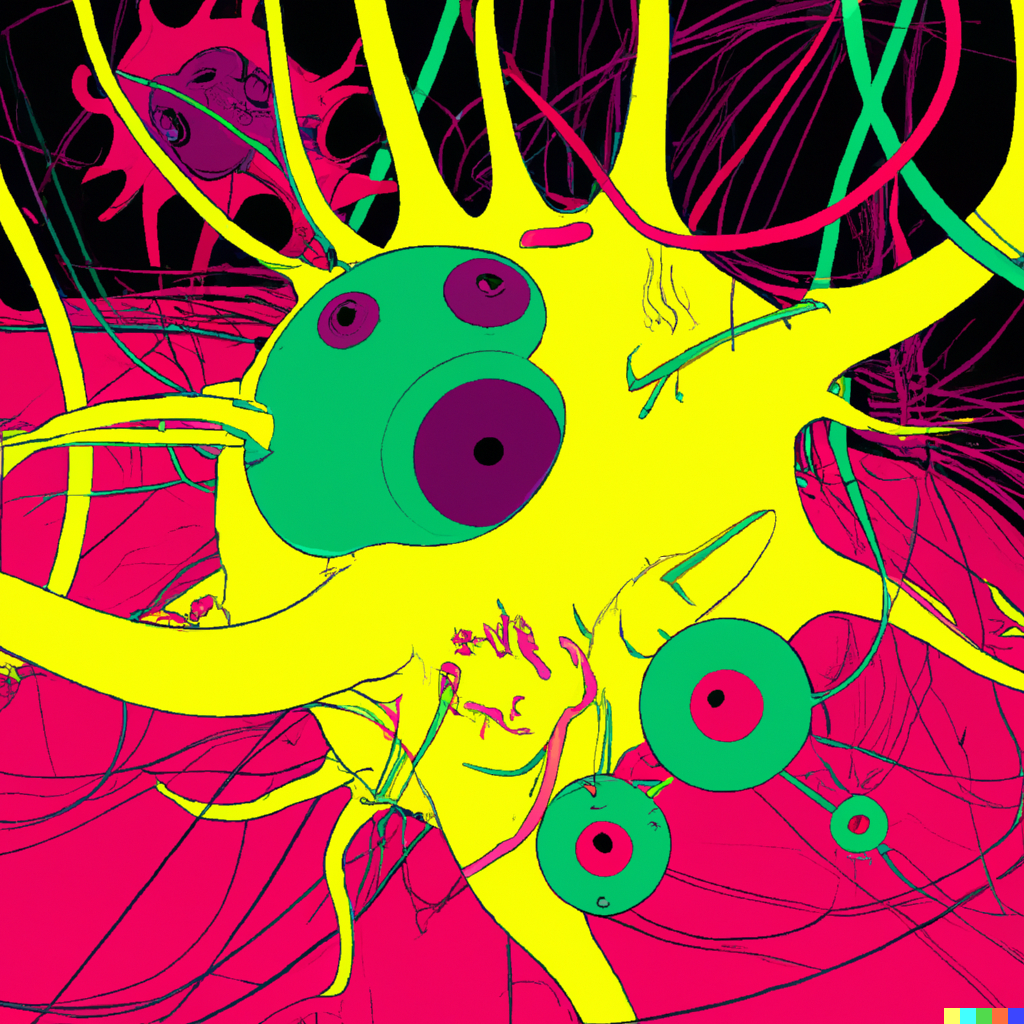
\includegraphics[width=0.4\textwidth]{fig}
\end{center}

Given the $N$ bacteria in the Petri dish, your starting size $S$, and a number of hours $H$, determine the maximum size you can reach after $H$ hours.


\section*{Input}

The first line of input contains three integers, $N$~($1 \leq N \leq 300\,000$), $S$~($1 \leq S \leq 10^6$), and $H$~($1 \leq H \leq N$), which describe the number of bacteria, your starting size, and the number of hours, respectively. The next line contains $N$ integers each in the inclusive range from $1$ to $10^6$. These describe the sizes of the bacteria in the Petri dish other than yourself. There may be multiple bacteria with the same size.


\section*{Output}

Display the maximum size you can achieve after $H$ hours.
